\documentclass[acmsmall]{acmart}
\bibliographystyle{ACM-Reference-Format}

\usepackage{array}
\usepackage{tikz}
\usetikzlibrary{positioning}
\usepackage{pgfplots}
\pgfplotsset{compat=1.12}
\usepackage{siunitx}
\usepackage{todonotes}

\title{JuliaPetra: An Implementation of the Petra Object Model in Julia}

\author{Neil Lindquist}
\email{nslindquist@csbsju.edu}

\acmJournal{TOMS}


\newcommand{\snippet}[1]{\texttt{\detokenize{#1}}}

\begin{document}
	
	%REVIEW "Distributed algorithms → Self-organization" concept displayed as "self-organization"
	%TODO make sure the concepts represent what I think they do
	\begin{CCSXML}
		<ccs2012>
		<concept>
		<concept_id>10002950.10003714.10003715.10003719</concept_id>
		<concept_desc>Mathematics of computing~Computations on matrices</concept_desc>
		<concept_significance>500</concept_significance>
		</concept>
		<concept>
		<concept_id>10002950.10003705</concept_id>
		<concept_desc>Mathematics of computing~Mathematical software</concept_desc>
		<concept_significance>100</concept_significance>
		</concept>
		<concept>
		<concept_id>10010147.10010148.10010149.10010158</concept_id>
		<concept_desc>Computing methodologies~Linear algebra algorithms</concept_desc>
		<concept_significance>500</concept_significance>
		</concept>
		<concept>
		<concept_id>10010147.10010919.10010172.10003824</concept_id>
		<concept_desc>Computing methodologies~Self-organization</concept_desc>
		<concept_significance>100</concept_significance>
		</concept>
		</ccs2012>
	\end{CCSXML}
	
	\ccsdesc[500]{Mathematics of computing~Computations on matrices}
	\ccsdesc[100]{Mathematics of computing~Mathematical software}
	\ccsdesc[500]{Computing methodologies~Linear algebra algorithms}
	\ccsdesc[100]{Computing methodologies~Self-organization}
	
	\begin{abstract}
		JuliaPetra provides linear algebra data structures that are commonly used in large scale, linear solver algorithms.
		The data structures in JuliaPetra focus on vectors and sparse matrices, in both serial and
		distributed, parallel environments.
		The library is written in Julia, a high level programming language with comparable performance to C or Fortran.
		JuliaPetra performs as fast as Epetra, an equivalent C++ library, and faster than DistributedArrays.jl, a Julia
		library for distributed computations on arrays.
	\end{abstract}
	
	\maketitle
	
	\section{Introduction}
	
	JuliaPetra is an implementation of the Petra object model in Julia.
	The Petra object model is the design used in Trilinos for objects commonly used by linear solver algorithms
	\cite{Heroux:2005:Trilinos}.
	Petra libraries provide parallel, distributed matrices, vectors and graphs for other packages to use.
	By providing a set of interfaces for basic linear algebra structures, Petra libraries provide a way
	to develop packages for these types of distributed algorithms that are able to interact and build on each other.
	The Petra object model has previously been implemented in both C++ and Java.
	%REVIEW should this list of previous implemenetations be in the paper?
	
	%REVIEW does there need to be a section on Julia?
	%There isn't really an equivalent in papers for Fortrain/C programs
	%Julia is less estabilished for hpc though
	Julia is a programing language that uses just in time compiling and powerful type inferencing
	to obtain the speed of a statically compiled programing language with the productivity of an
	interpreted programing language \cite{Bezanson:2017:FreshApproach}.
	By providing speed comparable to that of Fortran or C, Julia is a candidate for doing large scale,
	high performance computations.
	The Celeste project is an example of large scale computations in Julia,
	using 8,192 cores of the Cori Supercomputer
	at Lawrence Berkeley National Laboratory \cite{Bezanson:2017:FreshApproach}.
	
	%REVIEW this is a strange paragraph.
	Like other implementations of the Petra object model,
	JuliaPetra provides the ability to do basic linear algebra computations.
	These computations include dot products, vector norms and sparse matrix - vector multiplications.
	This document provides, first, an overview of the types and interfaces of JuliaPetra,
	second, a summary of optimizations used to implement JuliaPetra,
	and finally, comparisons with two similar libraries, Epetra and DistributedArrays.jl.
	
	\section{The Petra Object Model}
	
	\todo[inline]{
		A general discussion of the Petra Object model, along with class diagrams.
	}
	
	\section{Design of JuliaPetra}
	
	The design of JuliaPetra follows closely with that of the C++ implementations of the
	Petra object model, Epetra and Tpetra.
	Like Epetra and Tpetra, JuliaPetra uses MPI and Single-Program-Multiple-Data as its base parallel model.
	The API is split into three main layers of abstraction, the communication layer, the problem distribution layer and the data structures layer.
	
	The first level of abstraction handles actual communication between processes.
	The \snippet{Comm} and \snippet{Distributor} types provide a low level interface to support different communication methods.
	Because all interprocess communication is done through these objects, new communication systems can be implemented without affected the objects built on top of the communication layer.
	There are two existing implementations of this layer, a serial implementation, with a trivial implementation, and an MPI implementation, built on MPI.jl~\cite{Github:MPI}.
	This communication layer provides the abstraction to build Single-Program-Multiple-Data logic without regard for the underlying communication implementation.
	
	The next layer of abstraction manages how the problem is distributed across processes.
	The \snippet{BlockMap}, \snippet{Directory}, \snippet{Import} and \snippet{Export}
	types handle the distribution of the problem across the processors.
	\snippet{BlockMap} and \snippet{Directory} manage which processor the various parts of
	the problem are located.
	\snippet{Import} and \snippet{Export} contain the logic behind redistributing
	the problem among the processes.
	The \snippet{SrcDistObject} and \snippet{DistObject} interfaces provide a connection between
	the redistributing logic and the data structures themselves.
	This provides an abstraction on which the distributed data structures can build.
	
	The linear algebra objects are built on top of the abstractions provided by the problem distribution layer.
	JuliaPetra has two main linear algebra types.
	The first type is the abstract type \snippet{MultiVector} which holds one or more vectors.
	This type is implemented by \snippet{DenseMultiVector} which stores dense vectors.
	The second type is the \snippet{Operator} interface which is implemented by types that provide a
	\(y \gets \alpha\cdot A(x) + \beta\cdot y\) operation, where \(\alpha\) and \(\beta\) are scalars,
	\(x\) and \(y\) are vectors and \(A\) is the operator.
	The abstract type \snippet{RowMatrix}, which stores sparse matrices accessed by rows,
	supports this interface by multiplying the matrix on the left of \(x\).
	\snippet{RowGraph} is an additionally type used to represent the sparsity pattern of a \snippet{RowMatrix}.
	Both \snippet{RowMatrix} and \snippet{RowGraph} have concrete implementations based on
	compressed sparse row format, \snippet{CSRMatrix} and \snippet{CSRGraph} respectively.
	Julia's \snippet{AbstractArray} is subtyped by both the \snippet{MultiVector}
	and \snippet{RowMatrix} types to allow existing Julia code to interact with data in JuliaPetra objects.
	
	\begin{figure}
		%name, type, location
		\newcommand{\typeNode} [3]{\node[#2] (#1) [#3] {\snippet{#1}};}
		\newcommand{\explicitInheritance}[2]{\draw[->] (#1.south) -- (#2);}
		\newcommand{\implicitInheritance}[2]{\draw[dashed,->] (#1.south) -- (#2);}
		\begin{tikzpicture}[
		ImplicitInterface/.style={rectangle, draw=black, dashed, minimum size=5mm},
		ExplicitInterface/.style={rectangle, draw=black, minimum size=5mm},
		ConcreteType/.style={rectangle, draw=black, very thick, minimum size=5mm}
		]
		
		\typeNode{Comm}{ExplicitInterface}{}
		
		\typeNode{MPIComm}{ConcreteType}{below=.75cm of Comm}
		\explicitInheritance{Comm}{MPIComm.north}
		
		\typeNode{SerialComm}{ConcreteType}{right=.25cm of MPIComm}
		\explicitInheritance{Comm}{SerialComm.north}
		
		\typeNode{LocalComm}{ConcreteType}{left=.25cm of MPIComm}
		\explicitInheritance{Comm}{LocalComm.north}
		
		\typeNode{Distributor}{ExplicitInterface}{left=5.1cm of Comm}
		
		\typeNode{SerialDistributor}{ConcreteType}{below right=.75cm and -1cm of Distributor}
		\explicitInheritance{Distributor}{SerialDistributor.north}
		
		\typeNode{MPIDistributor}{ConcreteType}{left=.25cm of SerialDistributor}
		\explicitInheritance{Distributor}{MPIDistributor.north}
		
		
		
		\typeNode{Directory}{ExplicitInterface}{below right=.75cm and -1.25cm of MPIDistributor}
		
		\typeNode{BasicDirectory}{ConcreteType}{below=.75cm of Directory}
		\explicitInheritance{Directory}{BasicDirectory.north}
		
		\typeNode{BlockMap}{ConcreteType}{right=of Directory}
		
		\typeNode{Import}{ConcreteType}{right=of BlockMap}
		
		\typeNode{Export}{ConcreteType}{right=of Import}
		
		
		
		\typeNode{SrcDistObject}{ImplicitInterface}{below left=.75cm and -.9cm of Export}
		
		\typeNode{DistObject}{ImplicitInterface}{below=.75cm of SrcDistObject}
		\implicitInheritance{SrcDistObject}{DistObject.north}
		
		\typeNode{Operator}{ImplicitInterface}{left=of DistObject}
		
		\typeNode{AbstractArray}{ExplicitInterface}{left=of Operator}
		
		\typeNode{MultiVector}{ExplicitInterface}{below=of AbstractArray}
		\implicitInheritance{DistObject}{MultiVector.north east}
		\explicitInheritance{AbstractArray}{MultiVector.north}
		
		\typeNode{DenseMultiVector}{ConcreteType}{below=.75cm of MultiVector}
		\explicitInheritance{MultiVector}{DenseMultiVector.north}
		
		\typeNode{RowMatrix}{ExplicitInterface}{below=of Operator}
		\implicitInheritance{DistObject}{RowMatrix.north east}
		\implicitInheritance{Operator}{RowMatrix.north}
		\explicitInheritance{AbstractArray}{RowMatrix.north west}
		
		\typeNode{RowGraph}{ExplicitInterface}{below=of DistObject}
		\implicitInheritance{DistObject}{RowGraph.north}
		
		\typeNode{CSRMatrix}{ConcreteType}{below=.75cm of RowMatrix}
		\explicitInheritance{RowMatrix}{CSRMatrix.north}
		
		\typeNode{CSRGraph}{ConcreteType}{below=.75cm of RowGraph}
		\explicitInheritance{RowGraph}{CSRGraph.north}
		
		
		
		\node[ExplicitInterface] (ExplicitKey) [below=of CSRMatrix] {Abstract Type};
		\node[ImplicitInterface] (ImplicitKey) [left=of ExplicitKey] {Implicit Type};
		\node[ConcreteType]      (ConcreteKey) [right=of ExplicitKey] {Concrete Type};
		
		\end{tikzpicture}
		\Description{The key hierarchy of note is how \snippet{MultiVector}, \snippet{RowMatrix} and \snippet{RowGraph} implement the implicit type \snippet{DistObject} and both \snippet{MultiVector} and \snippet{RowMatrix} are subtypes of Julia's \snippet{AbstracyArray}.}
		\caption{Type Hierarchy.}
		\label{fig:type-hierarchy}
	\end{figure}
	
	The type hierarchy in JuliaPetra is limited by the fact that types in Julia are restricted to a single supertype.
	Interacting with existing code as a 2-dimensional array requires being a subtype of \snippet{AbstractArray}.
	So, the other interfaces for the data structures are not explicit types,
	but simply contracts promised in the documentation.
	These implicit interfaces include \snippet{Operator}, \snippet{SrcDistObject}
	and \snippet{DistObject}.
	%TODO consider discussing the vagueness of the definition of (Src)DistObject
	So, any methods that use one of those types accepts an object of any type
	and the documentation specifies the methods that must be implemented.
	Figure~\ref{fig:type-hierarchy} shows the full type hierarchy.
	
	\section{Optimizations of JuliaPetra}
	%This is to give insight on best practices for people who don't look at the general Julia discussions
	%Talk about the "story" of improving the code and how optimizations improved performance.
	
	There were alot of optimizations used to optimize JuliaPetra,
	many of which are standard adivice for optimizing Julia, such as type stability,
	or for optimization in general, such as accessing arrays in memory order.
	The only major unusual optimization was using \snippet{Ptr} objects to pass views of arrays
	in an effort to reduce allocation and garbage collection.
	
	The main improvements to performance in JuliaPetra came from improving type stability.
	Type stability is where the compiler can inference the types of all values.
	This allows the compiler is able to fully inline function calls, especially arithmetic and array operations.
	Because Julia is designed to support both slower, type unstable code and faster, type stable code,
	unlike C++ which is restricted to type stable code, some effort needs to be put into verifying
	type stability of performance critical code \cite{Bezanson:2017:FreshApproach}.
	%REVIEW mention that this is standard Julia advice?
	Removing type instabilities from performance critical sections of JuliaPetra improved performance
	by a few orders of magnitude.
	The \snippet{code_warntype} function was an important tool in finding type instabilities.
	Due to \snippet{code_warntype} requiring manual inspection, the TypeStability.jl library was created
	based on \snippet{code_warntype} to automatic type stability checks.
	
	Another notable optimization came from using \snippet{Ptr} objects to pass views of arrays.
	Because Julia is a garbage collected language, most objects in Julia must be allocated on the heap,
	then garbage collected when they are no longer used.
	However, certain objects, such as integers and floating point numbers can be allocated on the stack,
	so they don't need garbage collection.
	%needs some citations here
	So, by passing \snippet{Ptr} objects, which can be stack allocated,
	instead of \snippet{SubArray} objects, which must be heap allocated,
	the heap allocations and garbage collection can be greatly reduced in some performance critical sections
	However, this prevents use of higher level interfaces that Julia normally provides,
	such as the array length being stored with the array its self.
	This had much less of a performance increase that improving type stability,
	however, it is not a standard optimization for Julia so it deserved mention.
	
	Other, common and minor optimizations were also made.
	This optimizations include skipping unnecessary bounds checks
	and ensuring arrays data was accessed in the order it is stored in memory.
	Additionally, function calls in frequently used loops were replaced with specialized, inlined versions
	that take into account the context of the calling method
	and avoid using generalized methods that produce extra computations.
	%REVIEW should I go into more detail on the specific example (getting a row in SpMV)
	
	\section{Comparisons with Other Distributed Libraries}
	
	\subsection{Comparison with Epetra}
	
	Epetra is the base implementation of the Petra object model,
	written in a stable subset of C++ \cite{Heroux:2005:Trilinos}.
	Because Epetra was used as a template for implementing JuliaPetra,
	the APIs for JuliaPetra are similar to those for Epetra.
	The similarities between JuliaPetra and Epetra can be seen in how similar the respective implementations
	of the power method are.
	The differences in features between the implementation languages result in differences
	between JuliaPetra's and Epetra's APIs.
	For example, JuliaPetra takes advantage of higher level structures
	such as type templating and thrown exceptions.
	
	JuliaPetra is able to achieve the same performance as Epetra on large instances of the power method,
	as shown in Table~\ref{tab:timing-results}.
	Since Julia uses just in time compiling, the JuliaPetra power method has extra start up costs compared to
	the Epetra version. However, since each specialized method needs to be compiled only once,
	this is a fixed cost during the first evaluation.
	Additionally, JuliaPetra uses runtime dispatch in a few locations, such as with
	\snippet{Comm} objects, which adds additional overhead compared to Epetra.
	
	\subsection{Comparison with DistributedArrays.jl}
	
	DistributedArrays.jl is a similar library to JuliaPetra that supports
	distributed arrays in parallel environments \cite{Github:DA}.
	It uses Julia's built in fork-and-join model for parallelism
	\cite{Bezanson:2017:FreshApproach}.
	DistributedArrays.jl offers a number of usability advantages over JuliaPetra, however, it is not able to match the speed of JuliaPetra.
	
	DistributedArrays.jl has advantages over JuliaPetra because it is better designed to function with
	existing Julia code.
	For example, it is built around the standard models of parallelization and arrays in Julia.
	Another advantage is that DistributedArrays.jl uses an instance of \snippet{AbstractArray}
	for a process's local storage, this allows automatic support for different array structures.
	Finally, by keeping the program logic on the master process, DistributedArrays.jl can be used to
	do distributed computations while using Julia's read-eval-print loop.
	
	However, DistributedArrays.jl is performs much worse for the sparse operations used in the comparison timings.
	This difference in performance likely stems from the fact that DistributedArrays.jl is optimized towards dense matrix operations, resulting in unnecessary communication and computation when working with sparse matrices.
	A Julia 0.6.0 version of DistributedArrays.jl was modified to be more conducive to sparse matrix operations, but that implementation was neither able to match the performance of JuliaPetra nor updated to the Julia 1.0 compatible version of DistributedArrays.jl.
	
	\subsection{Timing Results}
	
	\begin{table}
		\caption{Timing results of various power method implementations.  All times are in seconds.}
		\label{tab:timing-results}
		\begin{tabular}{|c c|S|S|S||S|}
			\hline
			\multicolumn{2}{|c|}{Equations Per Process}
			& {JuliaPetra}
			& {Epetra}
			& \multicolumn{1}{m{1.8cm}||}{Distributed\-Arrays.jl}
			& \multicolumn{1}{m{1.75cm}|}{JuliaPetra \(\div\) Epetra}\\
			\hline
			\multicolumn{6}{|l|}{4 Processors}\\
			
			\hline
			100,000			&Mean & 0.22850 & 0.18045 & 124.322 & 1.26633 \\
			equations		&Minimum & 0.22768 & 0.13394 & 123.324 & 1.69985 \\
			&Maximum & 0.22933 & 0.21588 & 126.464 & 1.06232 \\
			\hline
			1,000,000		&Mean & 2.82589 & 2.35860 & 1149.26 & 1.19812 \\
			equations		&Minimum & 2.80843 & 2.34777 & 1144.52 & 1.19621 \\
			&Maximum & 2.83711 & 2.36840 & 1162.54 & 1.19790 \\
			\hline
			10,000,000		&Mean & 30.7656 & 24.6991 & {-} & 1.24562 \\
			equations		&Minimum & 30.5471 & 24.5430 & {-} & 1.24464 \\
			&Maximum & 31.2470 & 24.7841 & {-} & 1.26077 \\
			\hline
			\multicolumn{6}{|l|}{16 Processors}\\
			\hline
			100,000			&Mean & 0.54401 & 0.55244 & 2569.82 & 0.98474 \\
			equations		&Minimum & 0.52902 & 0.50857 & 2525.37 & 1.04021 \\
			&Maximum & 0.55428 & 0.56908 & 2713.96 & 0.97400 \\
			\hline
			
			1,000,000		&Mean & 7.44313 & 7.43903 & {-} & 1.00055 \\
			equations		&Minimum & 7.41123 & 7.42147 & {-} & 0.99862 \\
			&Maximum & 7.53777 & 7.45056 & {-} & 1.01171 \\
			\hline
			10,000,000		&Mean & 73.4730 & 73.9551 & {-} & 0.99348 \\
			equations		&Minimum & 73.1307 & 73.9172 & {-} & 0.98936 \\
			&Maximum & 74.1664 & 73.9953 & {-} & 1.00231 \\
			\hline
			\multicolumn{6}{|l|}{20 Processors}\\
			\hline
			100,000			&Mean & 0.76502 & 0.72094 & {-} & 1.06114 \\
			equations		&Minimum & 0.73781 & 0.69893 & {-} & 1.05563 \\
			&Maximum & 0.79881 & 0.76437 & {-} & 1.04507 \\
			\hline
			1,000,000		&Mean & 9.67784 & 9.74738 & {-} & 0.99287 \\
			equations		&Minimum & 9.47876 & 9.61908 & {-} & 0.98541 \\
			&Maximum & 9.85454 & 9.86118 & {-} & 0.99933 \\
			\hline
			10,000,000		&Mean & 96.6538 & 97.4296 & {-} & 0.99204 \\
			equations		&Minimum & 95.1889 & 96.7890 & {-} & 0.98347 \\
			&Maximum & 97.5618 & 98.0169 & {-} & 0.99536 \\
			\hline
		\end{tabular}
	\end{table}
	
	\todo[inline]{
		The timing results could be a bit confusing to the reader.  It would be worth mentioning specifically what the total number of equations is, at least in the description.  Better notes on speedups could improve it.  Also, it would be good to get some timing results from something beyond a tridiagonal matrix.
	}
	
	As can be seen in Table~\ref{tab:timing-results}, JuliaPetra is very close to the performance of Epetra, except when only using a few processors.
	Additionally, JuliaPetra is able to significantly outperform DistributedArrays.jl.
	Note that the last column shows the ratio of the JuliaPetra time over the Epetra time; in other words, a higher ratio indicates that the same problem will take longer to solve using JuliaPetra compared to Epetra.
	Additionally, the number of iterations was consistant between all problems, meaning the number of operations completed is only a function of number of processes and local problem size.
	The sizes were chosen to test how the libraries respond to different local workloads and different communication loads.
	JuliaPetra is slower for problems with less communication, while close to Epetra to problems with more communication.
	This implies that JuliaPetra may be slower for the actual computations, but the communication for larger problems overcomes the difference or is more efficient in JuliaPetra.
	As can been seen in Figures~\ref{fig:result-localsize} and~\ref{fig:result-numproc}, the execution time relates close to linearly with the local problem size and slightly superlinear with the number of processes for both JuliaPetra and Epetra.
	
	\begin{figure}
		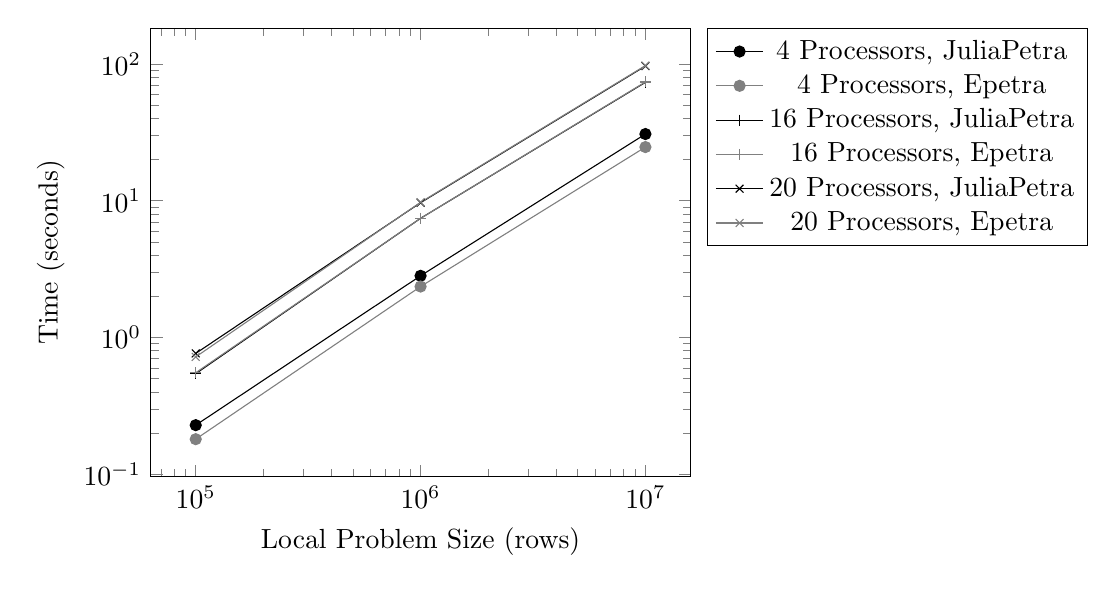
\begin{tikzpicture}
		\begin{loglogaxis}[
		xlabel = {Local Problem Size (rows)},
		ylabel = {Time (seconds)},
		legend pos = outer north east
		]
		\addplot[color=black,mark=*] coordinates{(100000,0.22850)(1000000,2.82589)(10000000,30.7656)};
		\addlegendentry{4 Processors, JuliaPetra}
		\addplot[color=gray,mark=*]  coordinates{(100000,0.18045)(1000000,2.35860)(10000000,24.6991)};
		\addlegendentry{4 Processors, Epetra}
		\addplot[color=black,mark=+] coordinates{(100000,0.54401)(1000000,7.44313)(10000000,73.4730)};
		\addlegendentry{16 Processors, JuliaPetra}
		\addplot[color=gray,mark=+]  coordinates{(100000,0.55244)(1000000,7.43903)(10000000,73.9551)};
		\addlegendentry{16 Processors, Epetra}
		\addplot[color=black,mark=x] coordinates{(100000,0.76502)(1000000,9.67784)(10000000,96.6538)};
		\addlegendentry{20 Processors, JuliaPetra}
		\addplot[color=gray,mark=x]  coordinates{(100000,0.72094)(1000000,9.74738)(10000000,97.4296)};
		\addlegendentry{20 Processors, Epetra}
		\end{loglogaxis}
		\end{tikzpicture}
		\Description{A graph of data from Table~\ref{tab:timing-results} showing approximately linear relation between the local problem size and the execution time.}
		\caption{Problem Size Versus Time for Various Numbers of Processors and Implementations.}
		\label{fig:result-localsize}
	\end{figure}
	
	\begin{figure}
		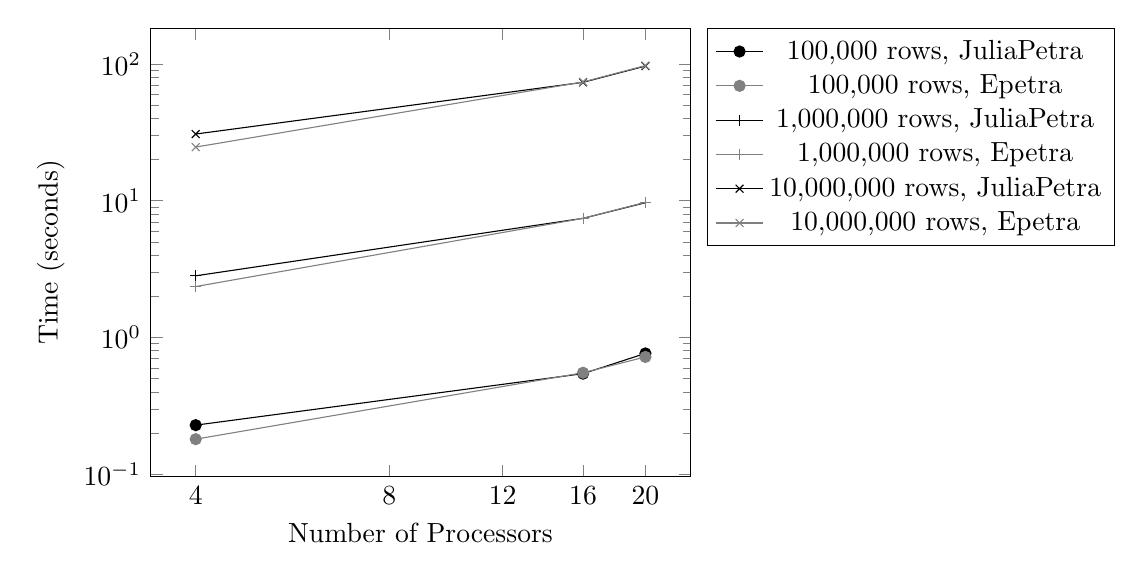
\begin{tikzpicture}
		\begin{axis}[
		ymode = log,
		xmode = log,
		xlabel = {Number of Processors},
		xtick = {4,8,12,16,20},
		xticklabels = {4,8,12,16,20},
		ylabel = {Time (seconds)},
		legend pos = outer north east
		]
		\addplot[color=black,mark=*] coordinates{(4,0.22850)(16,0.54401)(20,0.76502)};
		\addlegendentry{100,000 rows, JuliaPetra}
		\addplot[color=gray,mark=*]  coordinates{(4,0.18045)(16,0.55244)(20,0.72094)};
		\addlegendentry{100,000 rows, Epetra}
		\addplot[color=black,mark=+] coordinates{(4,2.82589)(16,7.44313)(20,9.67784)};
		\addlegendentry{1,000,000 rows, JuliaPetra}
		\addplot[color=gray,mark=+]  coordinates{(4,2.35860)(16,7.43903)(20,9.74738)};
		\addlegendentry{1,000,000 rows, Epetra}
		\addplot[color=black,mark=x] coordinates{(4,30.7656)(16,73.4730)(20,96.6538)};
		\addlegendentry{10,000,000 rows, JuliaPetra}
		\addplot[color=gray,mark=x]  coordinates{(4,24.6991)(16,73.9551)(20,97.4296)};
		\addlegendentry{10,000,000 rows, Epetra}
		\end{axis}
		\end{tikzpicture}
		\Description{A graph of data from Table~\ref{tab:timing-results} showing a slightly superlinear relation between the number of processors and the execution time.}
		\caption{Number of Processors Versus Time for Various Problem Sizes and Implementations.}
		\label{fig:result-numproc}
	\end{figure}
	
	The timings come from implementations of the power method for finding the largest eigenvalue of a matrix
	\cite{Gu:2000:PowerMethod}.
	Epetra's \texttt{petra\_power\_method} example is used as the Epetra implementation and the other implementations are translations of that code~\cite{Heroux:2005:Trilinos}.
	This tests the performance of vector dot product, vector L2-norm and sparse matrix-vector multiplication functionalities.
	The matrices used were various sizes of symmetric tridiagonal matrices, with the diagonal consisting of 2's
	and the off diagonals containing -1's, that were distributed over different numbers of processors.
	Each combination of implementation, problem size and number of processors was run five times
	and the average, minimum and maximum are presented.
	All implementations were run once before collecting the timings, to ensure all Julia code was
	compiled before the timing started.
	Additionally, the setup for the problems were not counted as part of the times.
	Note that the DistributedArrays.jl implementation took over an hour to find the eigenvalue for some problem sizes.
	Given the timings produced by the Petra implementations, these problems were not run to completion and left without a time on the table.
	
	The MPI implementation was MPICH version 3.2 with TCP used for all inter-process communication, with MPI.jl version 0.7.0 wrapping MPI for JuliaPetra.
	The Julia tests were run with the Julia v1.0.0 precompiled binary for Linux with the \snippet{-O3} flag enabled at run time.
	Version 0.5.1 of DistributedArrays.jl was used.
	The Epetra tests were compiled with GCC 4.8.5, the \snippet{-O3} flag and Trilinos 12.10.1.
	Tests were run on a Red Hat Enterprise Linux Workstation, version 7.3,
	with a 20 core Intel E5-2698 v4 CPU.
	
	\section{Conclusion}
	
	JuliaPetra is an implementation of the Petra object model in the Julia programming language.
	So, it provides an interface for distributed solver algorithms to interact and build on each other.
	Additionally, by performing at the same speeds as Epetra,
	it allows Julia to compete with C++ for these types of high performance computations.
	
	%REVIEW are there other things that should be discussed in the conclusion
	%It feels pretty short
	
	\bibliography{bibliography}
\end{document}
